\documentclass[conference]{IEEEtran}
\IEEEoverridecommandlockouts
% The preceding line is only needed to identify funding in the first footnote. If that is unneeded, please comment it out.
\usepackage{cite}
\usepackage{amsmath,amssymb,amsfonts}
\usepackage{amsthm}
\usepackage{algorithmic}
\usepackage{graphicx}
\usepackage{textcomp}
\usepackage{xcolor}
\def\BibTeX{{\rm B\kern-.05em{\sc i\kern-.025em b}\kern-.08em
    T\kern-.1667em\lower.7ex\hbox{E}\kern-.125emX}}

\usepackage{longtable}
\usepackage{rotating}
\usepackage{multirow}
\usepackage{makecell}


\makeatletter
\renewcommand{\maketag@@@}[1]{\hbox{\m@th\normalsize\normalfont#1}}%
\makeatother


\newtheorem{theorem}{Theorem}
\newtheorem{corollary}{Corollary}
\newtheorem{property}{Property}
\newtheorem{lemma}{Lemma}
\newtheorem{remark}{Remark}

\makeatletter
\renewcommand{\maketag@@@}[1]{\hbox{\m@th\normalsize\normalfont#1}}%
\makeatother


\begin{document}

\title{IRS-Enabled Covert and Reliable Communications: How Many Reflection Elements are Required?}

\author{\IEEEauthorblockN{Manlin~Wang\textsuperscript{\dag},~Bin~Xia\textsuperscript{\dag},~Yao~Yao\textsuperscript{\dag},~Zhiyong~Chen\textsuperscript{\dag}~and Jiangzhou~Wang\textsuperscript{\ddag}}
\IEEEauthorblockA{\textsuperscript{\dag}\textit{Department of Electronic Engineering, Shanghai Jiao Tong University, Shanghai, China} \\
\textsuperscript{\ddag}\textit{School of Engineering, University of Kent, Canterbury, U.K.}\\
Email: \textsuperscript{\dag}\{wangmanlin, bxia, sandyyao, zhiyongchen\}@sjtu.edu.cn,\textsuperscript{\ddag}j.z.wang@kent.ac.uk}
}

\maketitle

\begin{abstract}
Short-packet communications are applied to various scenarios where transmission  covertness and reliability are crucial due to the open wireless medium and finite blocklength. Although intelligent reflection surface (IRS) has been widely utilized to enhance transmission covertness and reliability, the question of how many reflection elements at IRS are required remains unanswered, which is vital to system design and practical deployment. The inherent strong coupling exists between the transmission covertness and reliability by IRS, leading to the question of intractability. To address this issue, the detection error probability at the warder and its approximation are derived first to reveal the relation between covertness performance and the number of reflection elements. Besides, to evaluate the reliability performance of the system, the decoding error probability at the receiver is also derived. Subsequently, the asymptotic reliability performance in high covertness regimes is investigated, which provides theoretical predictions about the number of reflection elements at IRS required to achieve a decoding error probability close to 0 with given covertness requirements. Furthermore, Monte-Carlo simulations verify the accuracy of the derived results for detection (decoding) error probabilities and the validity of the theoretical predictions for reflection elements. Moreover, results show that more reflection elements are required to achieve high reliability with tighter covertness requirements, longer blocklength and higher transmission rates.
\end{abstract}

\begin{IEEEkeywords}
Covert and reliable transmission, short-packet communications, intelligent reflecting surface
\end{IEEEkeywords}

\section{Introduction}
The fifth generation of mobile standards expands its focus into massive machine-type communication (mMTC) and ultra-reliable low-latency communication (uRLLC) \cite{intro_short1}. In addition to transmission throughput, reliability and latency, transmission security is also essential in these scenarios since vast amounts of confidential information are transferred over an open wireless medium.

To ensure high transmission security, covert communication has received extensive concerns, which prevents the transmission behaviors from being detected by warders\cite{intro_covert}. The information-theoretic limits of covert communications were established in \cite{intro_covert} first. Subsequently, extra uncertainty sources have been utilized to further enhance covert capacity, such as the full-duplex receiver and the collaborative jammer. In addition, to tackle the resource-consuming issue, intelligent reflection surface (IRS) has emerged as a cutting-edge technology for covert communications \cite{intro_IRS1}.

Recently, massive efforts have been devoted to exploiting the performance gain  by IRS in covert communications. By jointly optimizing the phase shifts at IRS and beamformers at the transmitter, favorable communication environments were established for covert communication in \cite{IRS3,IRS_single10}. Based on the above system, the transmission probability was also optimized in \cite{IRS_single8}, and full-duplex technology was combined in \cite{IRS_single7}. Furthermore, IRS-assisted covert communications were extended to relaying networks\cite{IRS1}, non-orthogonal multiple access systems \cite{IRS_single2} and unmanned aerial vehicle assisted systems \cite{IRS_UAV1}.

Noteworthily, in many mMTC and uRLLC applications such as industrial automation and remote surgery, stringent latency and high transmission reliability are also mandatory requirements, where short-packet communication is required to minimize the transmission latency. However, the above existing works \cite{IRS3,IRS_single8,IRS_single10,IRS_single7,IRS_single2,IRS_UAV1,IRS1} focus on the system design based on Shannon information-theoretic framework with infinite blocklength assumptions, and they ignore the transmission reliability constraints. Thus, the analytical method and results obtained by these works are ineffective and cannot be directly applied to short-packet transmission where both covertness and reliability are required. However, it is imperative to reveal the benefit brought by IRS for short-packet communications to guarantee transmission covertness and reliability. More specifically, the question of how many reflection elements at IRS are required to achieve covert and reliable transmission is critical for practical system deployment and is still an open issue.

To address this issue, in this paper, an IRS-enabled short-packet communication system against a multi-antenna warder is considered, and the number of required reflection elements is provided to guarantee transmission covertness and reliability. Specifically, to evaluate the system covertness and reliability performance, the average detection error probability at the warder and the average decoding error probability at the receiver are derived. Besides, to facilitate system analysis, concise approximation expression for detection error probability is also proposed in high covertness scenarios. Furthermore, we give a quantitative answer to the question that how many reflection elements are required to achieve a decoding error probability close to 0 with given covertness requirements even if the number of antennas at the warder is infinite. Finally, the analytical results are justified by the Monte-Carlo simulations, and the impacts of system parameters on the system performance are illustrated, which provides some insights for practical system design.




\emph{Notation}: Vectors and matrices are denoted by boldface lowercase and uppercase letters, respectively. ${\bf{A}}^T$ and ${\bf{A}}^H$ denote the  transpose and conjugate transpose of ${\bf{A}}$, respectively. $diag({\bf{p}})$ denotes a diagonal matrix whose diagonal elements consist of the elements in the vector ${\bf{p}}$. $\left\| {\cdot} \right\|$ and $\left|  \cdot  \right|$ denote the Frobenius norm and the absolute value, respectively. $\mathcal{C N}({\bf{\mu}}, {\bf{\Sigma}})$ denotes the complex Gaussian distribution with mean ${\bf{\mu}}$ and covariance ${\bf{\Sigma}}$. ${\Pr}(\cdot)$ denotes the probability of an event. $\mathcal{Q}(x)=\int_x^{\infty} \frac{1}{\sqrt{2 \pi}} \exp \left(-t^2 / 2\right) d t$ denotes the Q-function. $\Gamma \left( n \right) = \left( {n - 1} \right)!$ denotes the Gamma function, $\gamma(n, x)=\int_0^x e^{-t} t^{n-1} d t$ denotes the lower incomplete Gamma function, and $\Gamma(n, x)=\int_x^{\infty} e^{-t} t^{n-1} d t$ denotes the upper incomplete Gamma function. 

\section{Signal and Channel Model}
\begin{figure}
	\centering
	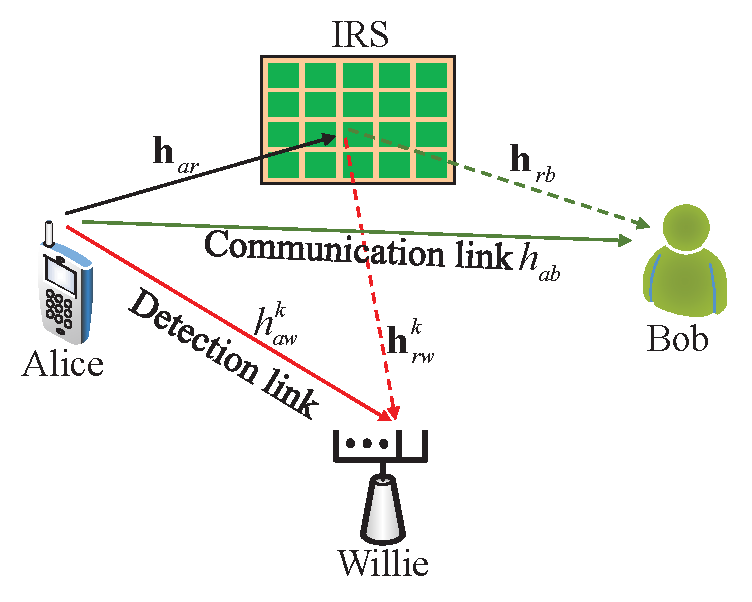
\includegraphics[width=0.85\linewidth]{figure/system.eps}
	\caption{IRS-enabled short-packet communication system against a multi-antenna warder.}
	\label{fig_sim}
\end{figure}
As shown in Fig. 1, a covert communication scenario is considered, where the transmitter (Alice) desires to deliver messages to the receiver (Bob) while keeping a multi-antenna warder (Willie) unaware of the transmission. Alice and Bob are assumed to be equipped with a single antenna, while Willie is assumed to be equipped with $N_w$ antennas. An IRS with $N_r$ reflection elements is deployed to assist this transmission.


In one transmission round, Alice transmits $n$ covert signals $x\left[ i \right] \sim \mathcal{CN}\left( {0,P_a} \right),i \in \left\{ {1, \ldots ,n} \right\}$ to Bob, where $P_a$ denotes the transmit power at Alice.  Willie collects $n$ received signals to detect whether the transmission happens or not. We denote the additive white Gaussian noise (AWGN) at Bob and Willie as ${{{n}}_b}\left[ i \right] \sim \mathcal{CN}\left( {0,\sigma _b^2} \right)$ and ${{\bf{n}}_w}\left[ i \right] \sim \mathcal{CN}\left( {{\bf{0}},\sigma_w^2{\bf{I}}} \right)$, where $\sigma_b^2$ and $\sigma_w^2$ are the noise variances at Bob and Willie, respectively.

The wireless channels from Alice to Bob ($h_{ab}$), from Alice to the $k$-th antenna of Willie (${{h}}_{aw,k}$), from Alice to IRS (${\bf{h}}_{ar}$), from IRS to Bob (${\bf{h}}_{rb}$), and from IRS to the $k$-th antenna of Willie (${\bf{h}}_{rw,k}$) are subject to the quasi-static Rayleigh fading \cite{IRS1}. The channel coefficients remain constant during one transmission round, and are independently and identically distributed (i.i.d.) among different rounds. Specifically, $h_{ab} \sim \mathcal{CN}(0,\lambda_{ab})$, $h_{aw,k} \sim \mathcal{CN}(0,\lambda_{aw})$, ${\bf{h}}_{ar} \sim \mathcal{CN}({\bf{0}},\lambda_{ar}{\bf{I}})$, ${\bf{h}}_{rb} \sim \mathcal{CN}({\bf{0}},\lambda_{rb}{\bf{I}})$, and ${\bf{h}}_{rw,k} \sim \mathcal{CN}({\bf{0}},\lambda_{rw}{{\bf{I}}})$. The instantaneous channel state information (CSI) of legitimate links (including the Alice-Bob link and Alice-IRS-Bob link) is assumed available at IRS by channel estimation \cite{channel_estimation}. In addition, since Willie does not cooperate with Alice, only statistical CSI of warder-related links (including the Alice-IRS-Willie link and Alice-Willie link) can be estimated at Alice through the local oscillator power inadvertently leaked from the receiver radio frequency frontend signal \cite{Willie_CSI3}. Besides, the instantaneous CSI of warder-related links is assumed available at Willie from the worst perspective for covert communication.

\section{Covertness Performance Analysis}
To detect the presence of covert communications, Willie must distinguish between the following two hypotheses
\begin{equation}
	{\bf{y}}_w[i]= \begin{cases} {\bf{n}}_w[i], & \mathcal{H}_0 \\ {\bf{h}}_w x[i]+{\bf{n}}_w[i], & \mathcal{H}_1\end{cases}
\end{equation}
where $\mathcal{H}_0$ and $\mathcal{H}_1$ denote the null hypothesis that Alice does not transmit and the alternative hypothesis that Alice transmits, respectively. ${\bf{y}}_w[i]$ is the received signal at Willie, and ${{\mathbf{h}}_w} = {\left[ {{h_{w,1}}, \ldots ,{h_{w,{N_w}}}} \right]^T}$ is the equivalent channel from Alice to Willie, where ${h_{w,k}} = {h_{aw,k}} + {\mathbf{h}}_{rw,k}^H{\mathbf{\Theta }}{{\mathbf{h}}_{ar}},k \in \left\{ {1, \ldots ,{N_w}} \right\}$. ${\mathbf{\Theta }} = diag\left( {{e^{j{\theta _1}}}, \ldots ,{e^{j{\theta _{{N_r}}}}}} \right)$ is the reflection matrix at IRS, where ${\theta _i} \in \left[ {0,2\pi } \right),i \in \left\{ {1, \ldots ,{N_r}} \right\}$ denotes the phase of $i$-th reflection element.

Considering the worst perspective for covert communication, when Willie knows the instantaneous CSI and the reflection coefficients at IRS, the maximum ratio combiner can be adopted as an optimal detector \cite{multi_antenna}
\begin{equation}
	T = \frac{1}{n}\sum\limits_{i = 1}^n {{{\left| {{{\bf{h}}_w^H}{{\mathbf{y}}_w}[i]} \right|}^2}} \mathop {\mathop  \gtrless \limits^{{\mathcal{D}_1}} }\limits_{{\mathcal{D}_0}} {\tau ^*},
\end{equation}
where $T$ is the average power of each received signal at Willie, $\mathcal{D}_1$ and $\mathcal{D}_0$ denote the binary decisions that infer whether Alice transmits or not, respectively. In addition, $\tau ^*$ denotes the optimal detection threshold, which is given by \cite{multi_antenna,hardware}
\begin{equation}\label{optimal_threshold1}
	{\tau ^*} = \frac{{\sigma _w^2\left( {\sigma _w^2 + {{\left\| {{{\mathbf{h}}_w}} \right\|}^2}{P_a}} \right)}}{{{P_a}}}\ln \left( {1 + \frac{{{{\left\| {{{\mathbf{h}}_w}} \right\|}^2}{P_a}}}{{\sigma _w^2}}} \right).
\end{equation}

Suppose there is no prior knowledge for Willie about when Alice will transmit. The prior probability of either hypothesis is equal. Mathematically, the detection error probability $\xi$ at Willie is defined as $	\xi=\operatorname{Pr}\left(\mathcal{D}_1 \mid \mathcal{H}_0\right)+\operatorname{Pr}\left(\mathcal{D}_0 \mid \mathcal{H}_1\right)$, where $ {\Pr}\left(\mathcal{D}_1 \mid \mathcal{H}_0\right)$ denotes the false alarm probability, and $ {\Pr}\left(\mathcal{D}_0 \mid \mathcal{H}_1\right)$ denotes the missed detection probability \cite{self3}. Thus, the minimum detection error probability $\xi^*$, with optimal detection threshold $\tau^*$. is expressed as \cite{linear}
\begin{equation}\label{Pd1}
	\begin{aligned}
		&\xi \left( {{\tau^* }} \right) = \Pr \left( {T > {\tau^* }|{H_0}} \right) + \Pr \left( {T < {\tau^* }|{H_1}} \right)\\
		& \!=\! 1 \!-\! \frac{1}{{\Gamma \!\left(\! n \!\right)\!}}\!\left(\! \!{\gamma \!\left(\!\! {n,\frac{{n{\tau ^*}}}{{{{\left\| {{{\mathbf{h}}_w}} \right\|}^2}\sigma _w^2}}} \!\right)\!\! -\! \gamma \!\left(\!\! {n,\!\frac{{n{\tau ^*}}}{{{{\left\| {{{\mathbf{h}}_w}} \right\|}^2}\sigma _w^2 \!+\! {{\left\| {{{\mathbf{h}}_w}} \right\|}^4}{P_a}}}} \!\right)\!} \!\right)\!.
	\end{aligned}
\end{equation}

Since Alice only knows the statistical CSI of warder-related links, the average detection error probability with statistical CSI is adopted as the covertness performance of the system.

\begin{theorem}
The average detection error probability at Willie with optimal	detection threshold can be derived as
	\begin{small}
	\begin{equation}\label{ave_Pd1}
	\begin{aligned}
		&{\overline \xi }\!\left( {{\tau ^*}} \!\right) \!=\! 1\!\!-\!\! \frac{\pi }{{B\Gamma \left( n \right)}}\sum\limits_{b = 1}^B {\!\left[\! {\gamma\! \left(\!\! {n,\!\frac{{n\left( {\sigma _w^2 \!+\! \tan {\theta _b}{P_a}} \right)}}{{\tan {\theta _b}{P_a}}}\!\ln\! \left(\!\! {\frac{{\sigma _w^2 \!+\! \tan {\theta _b}{P_a}}}{{\sigma _w^2}}} \!\!\right)\!} \!\!\right)\!\!} \right.}     \\
		&\left. { \!-\! \gamma\! \left(\! {n,\!\frac{{n\sigma _w^2}}{{\tan {\theta _b}{P_a}}}\!\ln \!\!\left(\! {\frac{{\sigma _w^2 \!+\! \tan {\theta _b}{P_a}}}{{\sigma _w^2}}} \!\!\right)\!} \!\right)\!} \!\right]\!\!\frac{{\sqrt {{\theta _b}\!\left(\! {\frac{\pi }{2} \!-\! {\theta _b}} \right)} {f}\left( {\tan {\theta _b}} \right)\!}}{{{{\cos }^2}{\theta _b}}},
	\end{aligned}
\end{equation}
\end{small}
where $B$ is the parameter of Gaussian-Chebyshev Quadrature, ${\theta _b} = \frac{\pi }{4}\left( {1 + \cos \frac{{\left( {2b - 1} \right)\pi }}{{2B}}} \right)$, and ${{f}}(x) = \frac{{{e^{ - \frac{x}{{{\lambda _w}}}}}{x^{{N_w} - 1}}}}{{\lambda _w^{{N_w}}\Gamma \left( {{N_w}} \right)}}$ with ${\lambda _w} = {\lambda _{aw}} + {N_r}{\lambda _{rw}}{\lambda _{ar}}$.
\end{theorem}

\begin{proof}
We denote ${X_k} = {\mathbf{h}}_{rw,k}^H{\mathbf{\Theta }}{{\mathbf{h}}_{ar}}$, which approximately follows the complex Gaussian distribution, i.e., ${X_k} \sim \mathcal{CN}\left( {0,{N_r}{\lambda _{rw}}{\lambda _{ar}}} \right)$, when $N_r$ is sufficiently large \cite{IRS_single2}. The tightness of this approximation is validated by \cite{IRS_single2} and Section VI even $N_r$ is relatively small. Thus, ${\left\| {{{\mathbf{h}}_w}} \right\|^2}$ follows the Gamma distribution with the probability density function (PDF) ${f}(x) = \frac{{{e^{ - \frac{x}{{{\lambda _w}}}}}{x^{{N_w} - 1}}}}{{\lambda _w^{{N_w}}\Gamma \left( {{N_w}} \right)}}$ \cite{multi_exp}. By substituting (\ref{optimal_threshold1}) into (\ref{Pd1}), the average detection error probability can be expressed as
	\begin{equation}\label{Pd1_int}
		\begin{aligned}
		&\overline \xi \left( {{\tau ^*}} \right) \!=\! 1 \!-\!\!\int\limits_0^\infty\! {\left[ {\gamma \!\left(\! {n,n\left( {\frac{{\sigma _w^2}}{{x{P_a}}} \!+\! 1} \right)\ln \!\left(\! {1 \!+\! \frac{{x{P_a}}}{{\sigma _w^2}}} \!\right)\!} \!\right)} \right.}  \\
		& \left. {  \!- \gamma \!\left(\! {n,\frac{{n\sigma _w^2}}{{x{P_a}}}\ln \!\left(\! {1 \!+\! \frac{{x{P_a}}}{{\sigma _w^2}}} \!\right)\!} \!\right)\!} \right]  \frac{{{f}(x)}}{{\Gamma \left( n \right)}}dx.
		\end{aligned}
	\end{equation}
By substituting $x = \tan \theta $ into (\ref{Pd1_int}) and applying Gaussian-Chebyshev Quadrature into the above integral expression \cite{Quadrature},  (\ref{ave_Pd1}) can be obtained, and the proof is completed.
\end{proof}

Due to the complicated form of (\ref{ave_Pd1}), it is intractable to guide the system design. To address this issue, we derive a tractable approximation of the detection error probability as follows.

\begin{lemma}
	In high covertness scenarios with moderate blocklength (such as $n \ge 50$), the average detection error probability at Willie can be approximated as
	\begin{equation}\label{ave_Pd2}
		{\bar \xi}\left( {{\tau ^*}} \right) \approx 1 - \sqrt {\frac{n}{{2\pi }}} \frac{{{N_w}{P_a}{\lambda_w}}}{{ {\sigma_w ^2}}}.
	\end{equation}
\end{lemma}
\begin{proof}
	The detection error probability (\ref{Pd1}) is approximated as 
	\begin{equation}
		\xi \left( {{\tau ^*}} \right)\mathop  \approx \limits^{(a)} 1 - \frac{{{e^{ - n}}{n^n}}}{{\Gamma \left( n \right)}}\frac{{{P_a}{{\left\| {{{\mathbf{h}}_w}} \right\|}^2}}}{{\sigma _w^2}}\mathop  \approx \limits^{(b)} 1 - \sqrt {\frac{n}{{2\pi }}} \frac{{{P_a}{{\left\| {{{\mathbf{h}}_w}} \right\|}^2}}}{{\sigma _w^2}},
	\end{equation}
	where step $(a)$ is obtained by the linear approximation in high covertness scenarios \cite{linear}, and step $(b)$ is due to $\mathop {\lim }\limits_{n \to \infty } \frac{{{e^{ - n}}{n^n}}}{{\Gamma \left( n \right)}} = \sqrt {\frac{n}{{2\pi }}} $ with relative error less than $2\times10^{-3}$ when $n \ge 50$.
	
Thus, the average detection error probability is derived as
	\begin{equation}\label{appendix1}
		\bar \xi \left( {{\tau ^*}} \right) \!\!\approx\!\!\!\!\!\!\!\!\!\! \int\limits_0^{\frac{{\sigma _w^2}}{{{P_a}}}\sqrt {\frac{{2\pi }}{n}} } \!\!\!\!\!\!\!\!{\left(\!\! {1 \!\!-\!\! \sqrt {\frac{n}{{2\pi }}}\! \frac{{{P_a}x}}{{\sigma _w^2}}} \!\right)\!} {f}\!\left(\! x \!\right)\!dx\!=\!1 \!-\! \sqrt {\frac{n}{{2\pi }}} \frac{{{N_w}{P_a}{\lambda _w}}}{{\sigma _w^2}} \!+\! {g_1}\!\left(\! {{P_a}} \!\right)\!,
	\end{equation}
	where ${g_1}\left( {{P_a}} \right) = \sqrt {\frac{n}{{2\pi }}} \frac{{{\lambda _w}{P_a}}}{{\Gamma \left( {{N_w}} \right)\sigma _w^2}}\Gamma \left( {{N_w} \!+\! 1,\frac{{\sigma _w^2}}{{{\lambda _w}{P_a}}}\sqrt {\frac{{2\pi }}{n}} } \right) \!-\! \frac{1}{{\Gamma \left( {{N_w}} \right)}}\Gamma \left( {{N_w},\frac{{\sigma _w^2}}{{{\lambda _w}{P_a}}}\sqrt {\frac{{2\pi }}{n}} } \right)$, which can be ignored compared with other terms due to $\mathop {\lim }\limits_{{P_a} \to 0} \frac{{{g_1}\left( {{P_a}} \right)}}{{{P_a}}} \!=\! 0$.
\end{proof}

The concise expression (\ref{ave_Pd2}) implies that the $\bar \xi(\tau^*)$ is linear to $\sqrt{n}$, $N_w$ and $P_a$ in high covertness scenarios, facilitating the performance analysis in Section V. Besides, the tightness of (\ref{ave_Pd2}) is also validated in Section VI.

\section{Reliability Performance Analysis}
When Alice transmits, the received signal at Bob is
\begin{equation}\label{y_b}
	{y_b}[i] = \left( {{h_{ab}} + {\mathbf{h}}_{rb}^H{\mathbf{\Theta }}{{\mathbf{h}}_{ar}}} \right)x[i] + {n_b}[i].
\end{equation}

Based on the received signal (\ref{y_b}), Bob can decode the messages. However, the decoding error can not be ignored due to finite blocklength, which is given by \cite{Q_app}
\begin{small}
\begin{equation}\label{Pout}
	\delta \left( {{\gamma _b}} \right) = \mathcal{Q}\left( {\frac{{\ln 2\sqrt n \left( {{{\log }_2}\left( {1 + {\gamma _b}} \right) - R} \right)}}{{\sqrt {1 - {{\left( {{\gamma _b} + 1} \right)}^{ - 2}}} }}} \right),
\end{equation}
\end{small}
where ${\gamma _b} = {{{{\left| {{h_{ab}} + {\mathbf{h}}_{rb}^H{\mathbf{\Theta }}{{\mathbf{h}}_{ar}}} \right|}^2}{P_a}} \mathord{\left/
		{\vphantom {{{{\left| {{h_{ab}} + {\mathbf{h}}_{rb}^H{\mathbf{\Theta }}{{\mathbf{h}}_{ar}}} \right|}^2}{P_a}} {\sigma _b^2}}} \right.
		\kern-\nulldelimiterspace} {\sigma _b^2}}$ denotes the received SNR at Bob, and $R$ is the transmission rate measured by bits per channel use (bpcu). Since the decoding error probability (\ref{Pout}) is affected by fading channels, the average decoding error probability $\overline \delta$ is adopted to evaluate the reliability performance.

IRS can adjust its reflection coefficients at each transmission round to maximize $\gamma_b$, where the optimal
phase is given by $\theta _i^* = \arg \left( {{h_{ab}}} \right) + \arg \left( {{h_{rb,i}}} \right) - \arg \left( {{h_{ar,i}}} \right)$, ${{h_{ar,i}}}$ and ${{h_{rb,i}}}$ denote the channel from Alice to the $i$-th element at IRS, and from the $i$-th element to Bob, respectively. Thus, the instantaneous SNR can be expressed as ${\gamma _b} = {{{X^2}{P_a}} \mathord{\left/
		{\vphantom {{{X^2}{P_a}} {\sigma _b^2}}} \right.
		\kern-\nulldelimiterspace} {\sigma _b^2}}$ where $X = \left| {{h_{ab}}} \right| + \sum\limits_{i = 1}^{{N_r}} {\left| {{h_{rb,i}}} \right|\left| {{h_{ar,i}}} \right|}$. According to \cite[Lemma 1]{short_IRS2}, $X$ can be approximated by a generalized Gamma distribution with PDF ${f_X}(x) = {{{\beta ^\alpha }{x^{\alpha  - 1}}{e^{ - \beta x}}} \mathord{\left/
		{\vphantom {{{\beta ^\alpha }{x^{\alpha  - 1}}{e^{ - \beta x}}} {\Gamma \left( \alpha  \right)}}} \right.
		\kern-\nulldelimiterspace} {\Gamma \left( \alpha  \right)}}$, where $\alpha  = {{{\Psi ^2}} \mathord{\left/
		{\vphantom {{{\Psi ^2}} \Phi }} \right.
		\kern-\nulldelimiterspace} \Phi }$, $\beta  = {\Psi  \mathord{\left/
		{\vphantom {\Psi  \Phi }} \right.
		\kern-\nulldelimiterspace} \Phi }$, $\Psi  = {{{\alpha _d}} \mathord{\left/
		{\vphantom {{{\alpha _d}} {{\beta _d}}}} \right.
		\kern-\nulldelimiterspace} {{\beta _d}}} + {N_r}{{{\alpha _r}} \mathord{\left/
		{\vphantom {{{\alpha _r}} {{\beta _r}}}} \right.
		\kern-\nulldelimiterspace} {{\beta _r}}}$, $\Phi  = {{{\alpha _d}} \mathord{\left/
		{\vphantom {{{\alpha _d}} {\beta _d^2}}} \right.
		\kern-\nulldelimiterspace} {\beta _d^2}} + {N_r}{{{\alpha _r}} \mathord{\left/
		{\vphantom {{{\alpha _r}} {\beta _r^2}}} \right.
		\kern-\nulldelimiterspace} {\beta _r^2}}$, ${\alpha _{{d}}} = \frac{\pi }{{4 - \pi }}$, ${\beta _{{d}}} = \frac{{2\sqrt \pi  }}{{(4 - \pi )\sqrt {{\lambda _{ab}}} }}$, ${\alpha _{{r}}} = \frac{{{\pi ^2}}}{{16 - {\pi ^2}}}$ and ${\beta _{{r}}} = \frac{{4\pi }}{{\left( {16 - {\pi ^2}} \right)\sqrt {{\lambda _{ar}}{\lambda _{rb}}} }}$. Then, the PDF of $\gamma_b$ is derived as
\begin{equation}
	{f_{{\gamma _b}}}(t) = \frac{{{\beta ^\alpha }{e^{ - \beta \sqrt {\frac{{\sigma _b^2t}}{{{P_a}}}} }}}}{{2\Gamma \left( \alpha  \right)t}}{\left( {\frac{{\sigma _b^2t}}{{{P_a}}}} \right)^{\frac{\alpha }{2}}},
\end{equation}
and the average decoding error probability can be derived as
\begin{small}
\begin{equation}\label{Pout1}
	\begin{aligned}
	&\bar \delta  \!=\! \int\limits_0^\infty  {\delta \left( t \right)} {f_{{\gamma _I}}}(t)dt\mathop  \approx \limits^{(a)} \int\limits_{\!\varpi  - \frac{1}{{2\nu }}}^{\varpi  + \frac{1}{{2\nu }}}\! {\!\nu\! {F_{{\gamma _I}}}\left( t \right)dt} \\
	&\!=\! \frac{{\gamma \!\left(\! {\alpha ,\beta \sqrt {\frac{{\sigma _b^2}}{{{P_a}}}\left( {\varpi  \!-\! \frac{1}{{2\nu }}} \!\right)\!} } \right)}}{{\Gamma \left( \alpha  \right)}} \!+\! g(\varpi  \!+\! \frac{1}{{2\nu }}) \!-\! g(\varpi  \!-\! \frac{1}{{2\nu }}),
	\end{aligned}
\end{equation}
\end{small}
where step $(a)$ is due to linear approximation of Q-function \cite{Q_app}, $\varpi  \!=\! {2^R} \!-\! 1$, $\nu  \!=\! \sqrt {\frac{n}{{2\pi \left( {{4^R} - 1} \right)}}} $, ${F_{{\gamma _b}}}\left( t \right) = \frac{1}{{\Gamma \left( \alpha  \right)}}\gamma \left( {\alpha ,\beta \sqrt {\frac{{\sigma _b^2t}}{{{P_a}}}} } \right)$ and $g(t) = \frac{{\nu {P_a}}}{{\Gamma (\alpha ){\beta ^2}\sigma _b^2}}\Gamma \left( {\alpha  + 2,\beta \sqrt {\frac{{\sigma _b^2t}}{{{P_a}}}} } \right) - \frac{{(2\varpi \nu  + 1)}}{{2\Gamma (\alpha )}}\Gamma \left( {\alpha ,\beta \sqrt {\frac{{\sigma _b^2t}}{{{P_a}}}} } \right)$.
\section{Theoretical Predictions about Required Reflection Elements}
In this section, the reliability performance is derived under the covertness requirement ${\overline \xi (\tau^*)} \geq 1 - \varepsilon $, where $\varepsilon$ is predetermined value to evaluate the covertness level. Besides, we provide the theoretical predictions about the number of reflection elements required to achieve a decoding error probability close to $0$ with given covertness requirements. 

On the one hand, $\bar \xi(\tau^*)$ decreases with $N_r$ as shown in (\ref{ave_Pd2}), which implies that the allowed transmit power $P_a$ also decreases with $N_r$ to meet the covertness requirement ${\overline \xi (\tau^*)} \geq 1 - \varepsilon $. On the other hand, $\bar\delta$ decreases with $N_r$ and $P_a$ as shown in (\ref{Pout1}). Therefore, the reliability guarantee by IRS is unclear but crucial, and the question that how many reflection elements are required to achieve a decoding error probability close to 0 with covertness requirements is significative.

To address this issue, we first derive the reliability performance in high covertness scenarios when $N_r \to \infty$ as follows.

\begin{theorem}\label{theorem_Pe_asy}
	When $N_r \to \infty$, the achievable average decoding error probability with given $\varepsilon$ in high covertness scenarios is
	\begin{equation}\label{tradeoff}
		\mathop {\lim }\limits_{{N_r} \to \infty }\!\!\!\! \overline \delta \!=\!\! \begin{cases} 1 ,\!\!\! &\!\! r_{rw}<r_1 \\
			\!{\frac{{(2\varpi \nu  + 1)}}{2} \!-\! \sqrt {\frac{{2\pi }}{n}} \frac{{{\pi ^2}\varepsilon \sigma _w^2{\lambda _{rb}}\nu {r_{rw}}}}{{16\sigma _b^2{\lambda _{rw}}}}},\!\!\! &\!\! {{r_1} \!\leqslant\! {r_{rw}} \!\!<\! {r_2}}\\
			0,\!\!\! &\!\! r_2 \leqslant r_{rw} \end{cases}
	\end{equation}
	where ${r_{rw}} = \mathop {\lim }\limits_{{N_r} \to \infty } \frac{{{N_r}}}{{{N_w}}}$ denotes the ratio of the number of reflection elements at IRS to that of antennas at Willie, ${r_1} = \sqrt {\frac{n}{{2\pi }}} \frac{{16{\lambda _{rw}}\sigma _b^2}}{{{\pi ^2}{\lambda _{rb}}\varepsilon \sigma _w^2}}\left( {\varpi  - \frac{1}{{2\nu }}} \right)$ and ${r_2} = \sqrt {\frac{n}{{2\pi }}} \frac{{16{\lambda _{rw}}\sigma _b^2}}{{{\pi ^2}{\lambda _{rb}}\varepsilon \sigma _w^2}}\left( {\varpi  + \frac{1}{{2\nu }}} \right)$.
\end{theorem}
\begin{proof}
	See Appendix \ref{proof_theorem5}.
\end{proof}

Theorem 2 gives the theoretical predictions about the number of reflection elements required to achieve high-reliability performance ($\bar\delta \!\to\! 0$) with $N_w \!\to\! \infty$. Specifically, when ${N_r} \!\ge\! r_2 {N_w}$, the decoding error probability approaches 0. However, when ${N_r} \!<\! r_1{N_w}$, the decoding error probability approaches 1. Besides, when ${r_1}{N_w} \!\le\! {N_r} \!<\! {r_2}{N_w}$, the decoding error probabilities approach values between 0 and 1. Moreover, it shows that the covertness requirements $\varepsilon$, the blocklength $n$ and the transmission rate $R$ all affect the critical factors $r_1$ and $r_2$. Specifically, the tighter the covert requirement, the longer the blocklength and the higher the transmission rate, the more reflection elements are required to guarantee high-reliability performance.

When the number of reflection elements at IRS (antennas at Willie) is finite, the decoding error probability can be obtained by substituting the maximum allowed transmit power ${P_a} = \sqrt {\frac{{2\pi }}{n}} \frac{{\sigma _w^2\varepsilon }}{{{N_w}{\lambda _w}}}$ by (\ref{ave_Pd2}) into (\ref{Pout1}). Finally, we summarize the achievable reliability of IRS-enabled short-packet communication systems under covertness requirements in Table I.

	
\begin{table}
		\begin{center}
			\caption{Achievable Decoding Error Probability}
			\begin{tabular}{|c|c|c|c|}
				\hline
				{Element Number} & {\makecell[c]{$N_w,N_r \!\!\to\!\! \infty$ \\ $r_{rw}<r_1$}} & {\makecell[c]{$N_w,N_r \!\!\to\!\! \infty$ \\ $r_1 \leq r_{rw}<r_2$}}&{\makecell[c]{$N_w,N_r \!\!\to\!\! \infty$ \\ $r_2 \leq r_{rw}$}}\\
				\hline
				\rule{0pt}{10pt}{$\bar\delta$} & 1 & (\ref{tradeoff}) & 0 \\
				\hline
				Element Number & {\makecell[c]{$N_w \!\!\to\!\! \infty$\\ $N_r$, finite}} & {\makecell[c]{$N_r \!\!\to\!\! \infty$ \\  $N_w$, finite}}&{\makecell[c]{$N_r, N_w$,\\ finite}}\\
				\hline
				\rule{0pt}{10pt}$\bar \delta$ & 1 & 0&(\ref{Pout1})\\
				\hline
			\end{tabular}
		\end{center}
		\vspace{-0.7cm}
	\end{table}

\section{Numerical Simulation}
In this section, numerical results are provided to evaluate the performance of IRS-enabled short-packet communications. For illustration, we assume that Alice, Bob, Willie, and the IRS are located at (0,0), (10m,0), (12m,-5m), and (10m,1m) in a two-dimensional plane, respectively. The fading parameters are expressed as ${\lambda _{ij}} \!=\! {\beta _0}{\left( {\frac{{{d_{ij}}}}{{{d_0}}}} \right)^{ - {\alpha _{ij}}}}\!, ij \in \left\{ {ab,ar,rb,aw,rw} \right\}$, where ${d_{ij}}$ denotes the distance between nodes $i$ and $j$,  ${d_{0}}=1$(m) is the reference distance, and ${\beta _0}=-30$(dB) denotes the channel power gain at the reference distance. And
${{\alpha _{ij}}}$ is the path loss exponents with ${\alpha _{ar}} = {\alpha _{rw}} = 2.2,{\alpha _{ab}} = {\alpha _{aw}} = 3.5,{\alpha _{rb}} = 2$. Besides, $\sigma_b^2=\sigma_w^2=-60$ (dBm), $R=0.2$ (bpcu) and $n=200$. All the simulation results presented are obtained by averaging over $10^{6}$ channel realizations.

\begin{figure}
	\centering
	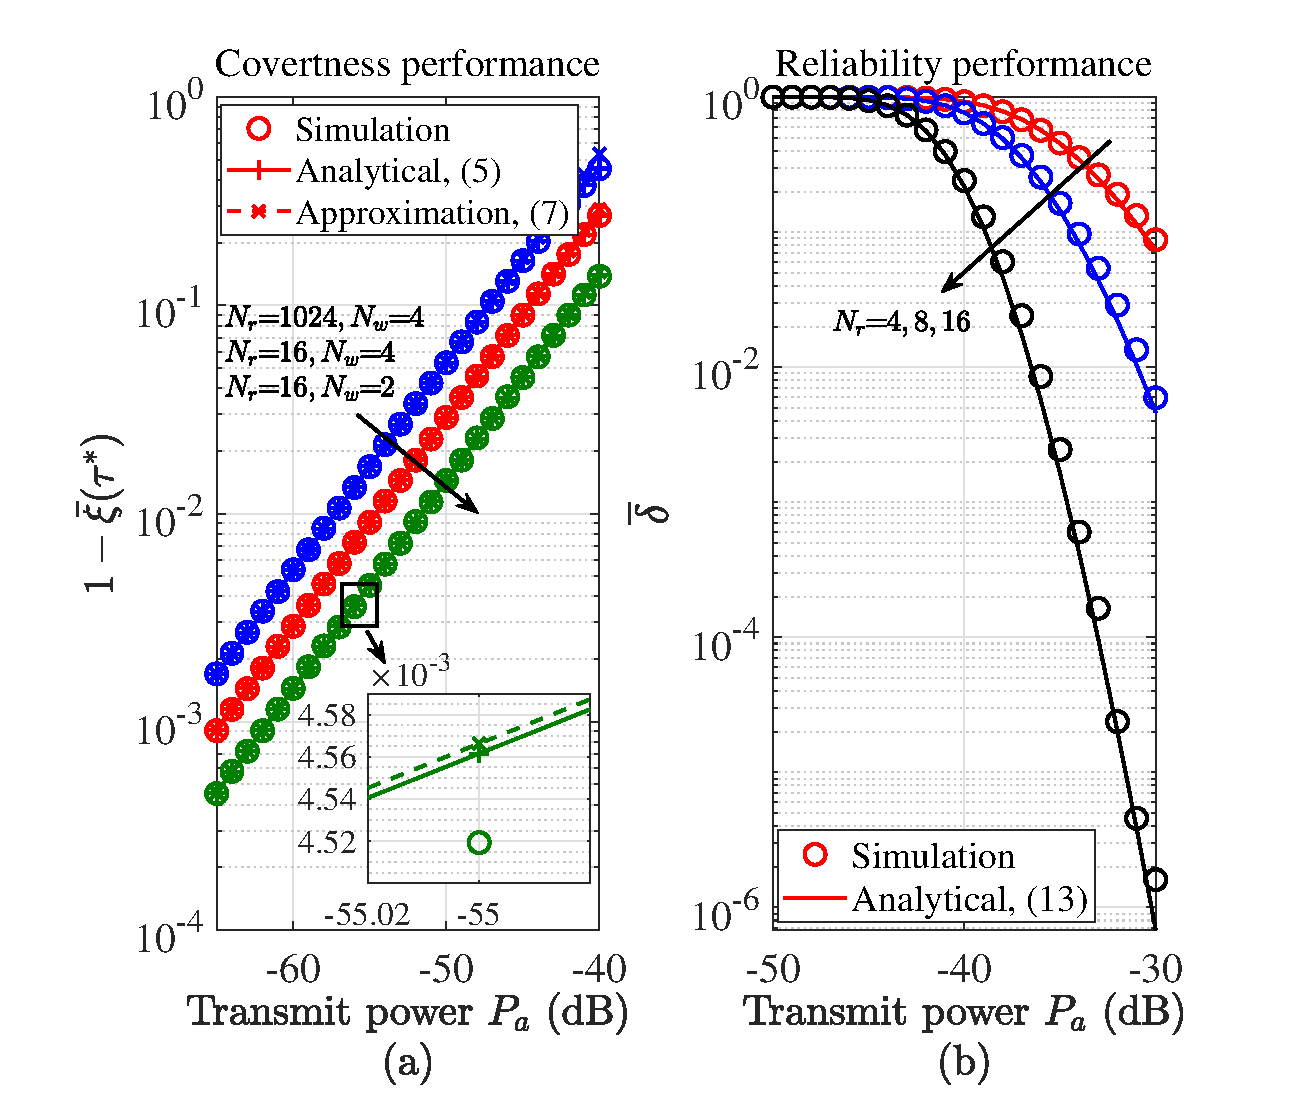
\includegraphics[width=0.85\linewidth]{figure/fig2_re.eps}
	\caption{The average detection error probability and decoding error probability versus the transmit power.}
\end{figure}
In Figs. 2 (a) and (b), the impacts of the transmit power on the average detection error probability and average decoding error probability are investigated. From Fig. 2 (a), it can be seen that the curves with numerical simulations, the analytical expression (\ref{ave_Pd1}), and the approximation expression (\ref{ave_Pd2}) coincide, even if the number of reflection elements is relatively small, such as $N_r\!\!=\!\!16$. From Fig. 2 (b), it can be seen that the results obtained by (\ref{Pout1}) are close to those obtained by numerical simulations, even if the number of reflection elements is relatively small, such as $N_r=4$. In addition, the detection (decoding) error probabilities decrease with $P_a$ and $N_r$ since more energy is received by Willie (Bob) when IRS is equipped with more reflection elements. These results validate the results given in Section III, implying that the proposed approximations (\ref{ave_Pd2}) and (\ref{Pout1}) can be adopted as covertness and reliability performance metrics due to their conciseness and tightness.

\begin{figure}
	\centering
	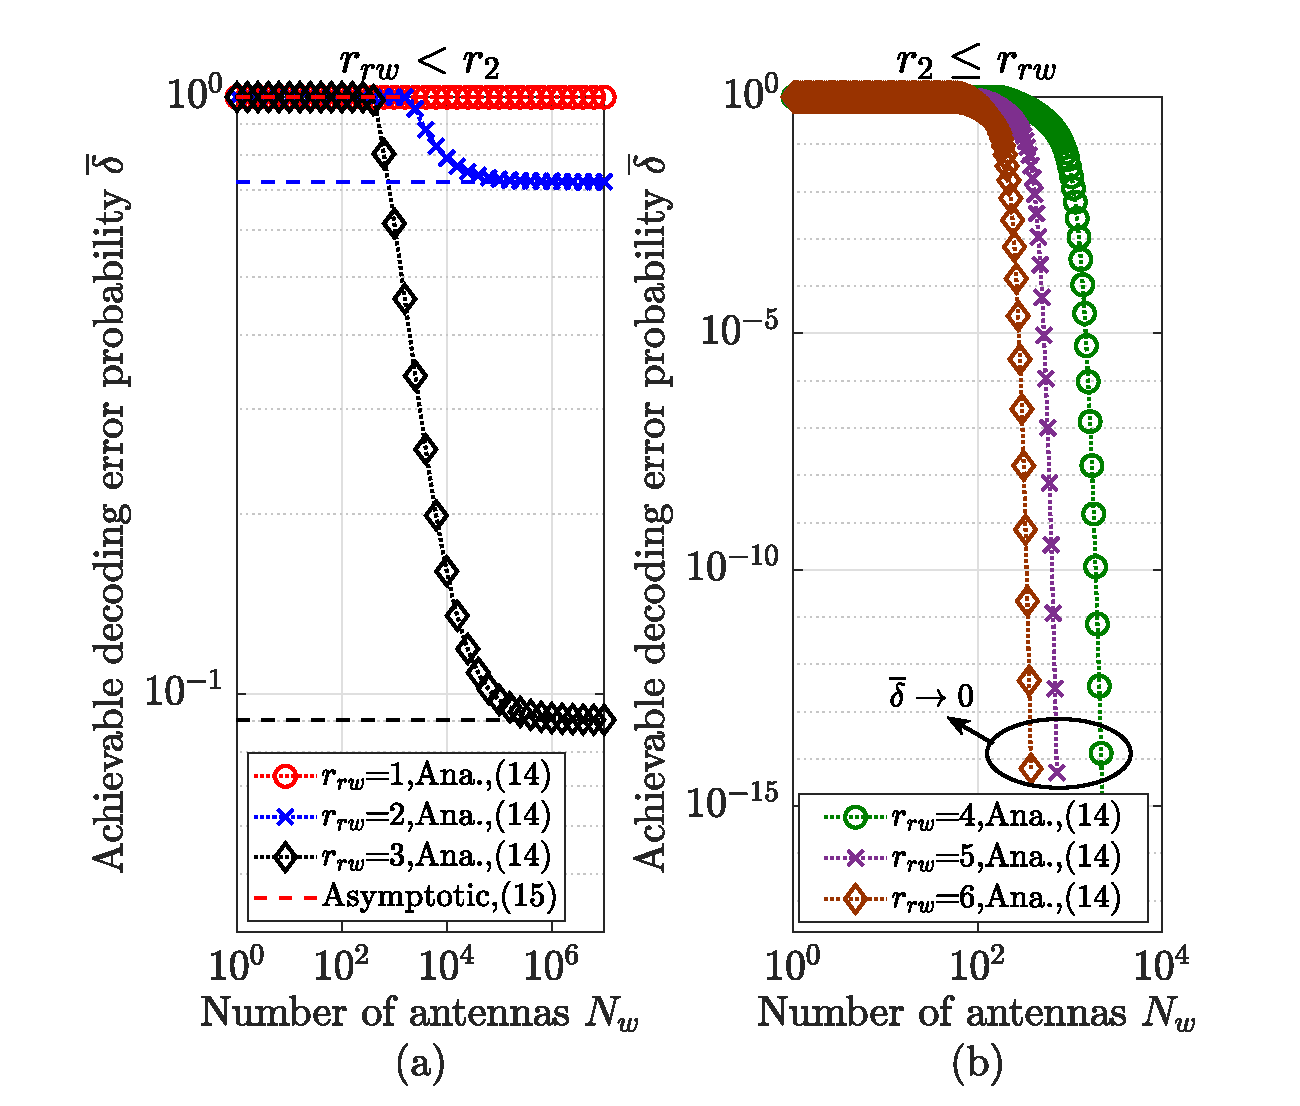
\includegraphics[width=0.85\linewidth]{figure/fig3_re.eps}
	\caption{The achievable decoding error probability versus the number of antennas at Willie.}
\end{figure}
In Figs. 3 (a) and (b), the impacts of the number of antennas and reflection elements on the decoding error probability are investigated, where the curves with “Ana.” denote the results obtained by (\ref{Pout1}). It can be seen that the results by (\ref{Pout1}) tend to the asymptotic ones by (\ref{tradeoff}) as $N_w,N_r \to \infty$. Specifically, from Fig. 5 (a), it can be seen that $\bar \delta \to 1$ when $r_{rw}=1<r_1=1.6$, and $\bar \delta \to 9\times10^{-2}$ when $r_1<r_{rw}=3<r_2=3.1$. Besides, from Fig. 5 (b), it can be seen that $\bar\delta \to 0$ , such as $\bar\delta<10^{-14}$ when $r_{rw}=4,5,6 \geq r_2=3.1$. These results verify the accuracy of Theorem 3, which gives the theoretical predictions that at least $r_2 N_w$ reflection elements at IRS are required for decoding error probabilities to approach 0.

\begin{figure}
	\centering
	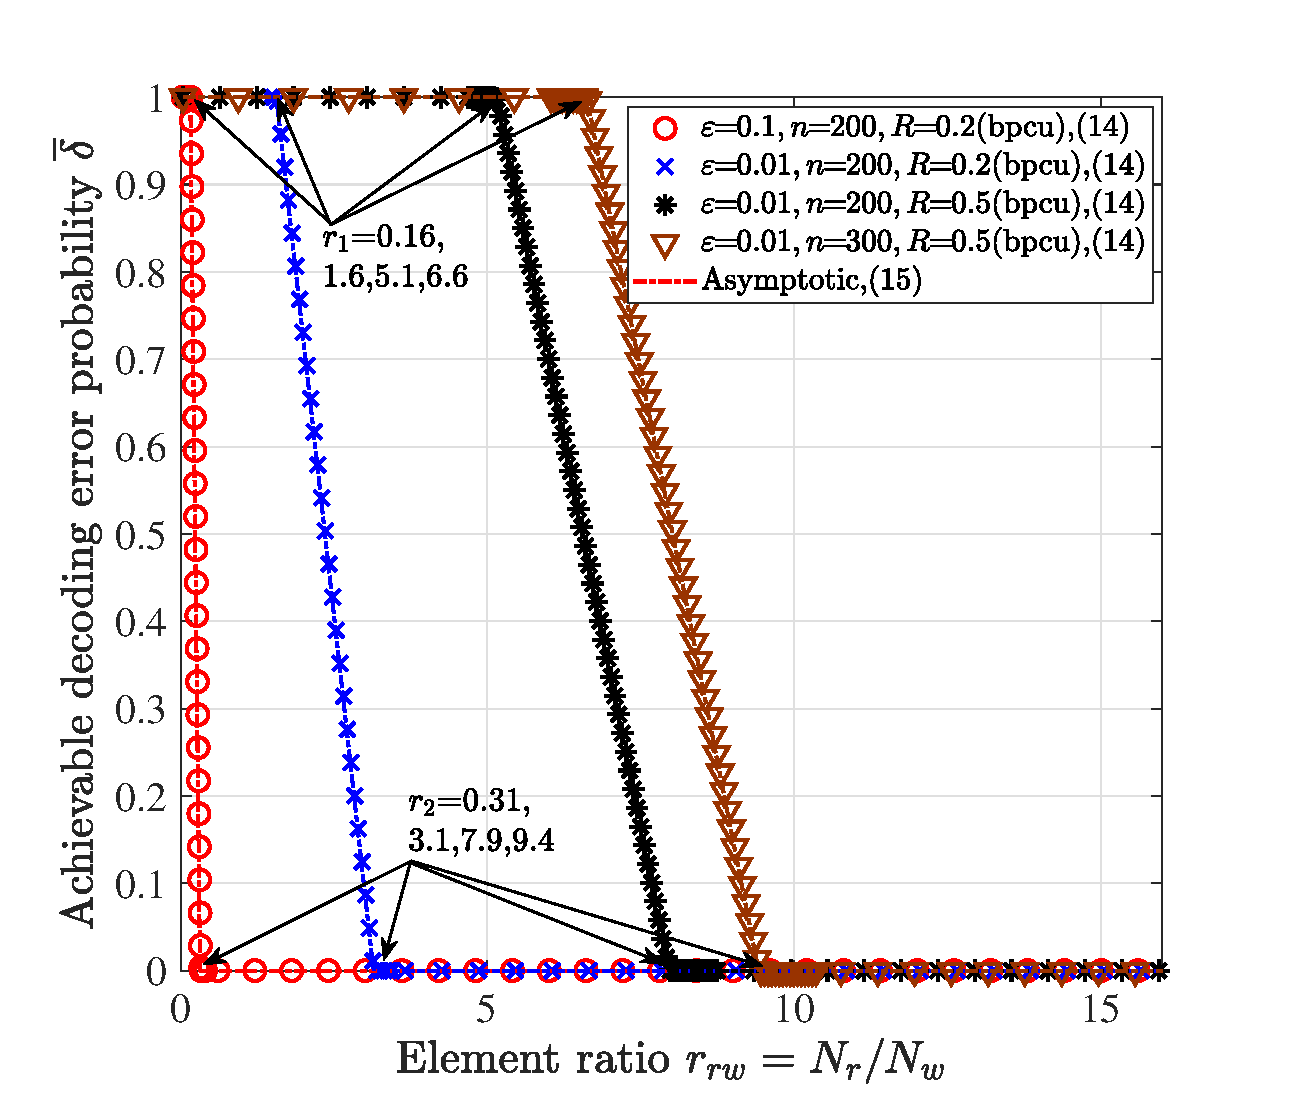
\includegraphics[width=0.85\linewidth]{figure/fig4_re.eps}
	\caption{The achievable decoding error probability versus the ratio $r_{rw}$.}
	\label{fig_sim}
\end{figure}
In Fig. 4, the impacts of system parameters on the decoding error probability are investigated, where the number of antennas at Willie is $10^6$. It can be seen that the results by (\ref{Pout1}) coincide with the asymptotic ones by (\ref{tradeoff}). Besides, it can be seen that the covertness requirements $\varepsilon$ and system parameters $n,R$ all affect the critical factors $r_1$ and $r_2$. Specifically, $r_1$ ($r_2$) changes from $0.16$ ($0.31$) to $1.6$ ($3.1$), when $\varepsilon$ changes from $0.1$ to $0.01$. Similarly, $r_1$ ($r_2$) changes from $1.6$ ($3.1$) to $5.1$ ($7.9$), when $R$ changes from $0.2$ (bpcu) to $0.5$ (bpcu). In addition, $r_1$ ($r_2$) changes from $5.1$ ($7.9$) to $6.6$ ($9.4$), when $n$ changes from 200 to 300. These results demonstrate that more reflection elements are required to achieve high reliability ($\bar\delta\!\to\!0$) with tighter covertness requirements, higher transmission rates and longer blocklength, which provides insights for the practical system design.


\section{Conclusion}
In this paper, we have provided the theoretical prediction about the required number of reflection elements to guarantee covertness and reliability performance in IRS-enabled short-packet communications. To this end,
the detection error probability at Willie has been derived firstly for evaluating the covertness performance, where a concise approximation is also provided to facilitate further analysis. Then, the decoding error probability at Bob has been derived for evaluating the reliability performance. Combined with the above system performance metrics, we have analyzed the required number of reflection elements at IRS to achieve high-reliability ($\bar\delta \to 0$) with covertness requirement $\bar\xi (\tau^*) \geq 1-\varepsilon$ in the asymptotic regime. Finally, Monte-Carlo simulations have been provided to evaluate the accuracy of analytical results and the validity of the theoretical predictions. Simulation results have shown that system parameters ($\varepsilon,n,R$) significantly affect the required number of refelction elements, which guides the system design.


\appendices
\section{Proof of Theorem 2}\label{proof_theorem5}
In high covertness scenarios with $N_r \to \infty$, the allowed transmit power with given covertness requirement $\varepsilon$ is  ${P_a} = \sqrt {\frac{{2\pi }}{n}} \frac{{\varepsilon \sigma _w^2}}{{{N_r}{N_w}{\lambda _{rw}}{\lambda _{ar}}}}$. Besides, when $N_r \to \infty$, $\alpha  \approx \frac{{{N_r}{\pi ^2}}}{{16 - {\pi ^2}}}$, $\beta  \approx \frac{{4\pi }}{{\left( {{{16 - }}{\pi ^2}} \right)\sqrt {{\lambda _{ar}}{\lambda _{rb}}} }}$. By substituting the allowed transmit power and above approximations into (\ref{Pout1}), we can obtain
\begin{small}
\begin{equation}
	\begin{aligned}
		\mathop {\lim }\limits_{{N_r} \to \infty } \!{{\bar \delta }}\! &=\! {f_2}(\varpi  \!-\! \frac{1}{{2\nu }}) \!+\! \left(\!\! {\sqrt {\frac{{2\pi }}{n}} \frac{{{N_r}{\pi ^2}\varepsilon \sigma _w^2{\lambda _{rb}}\nu }}{{16\sigma _b^2{N_w}{\lambda _{rw}}}} \!-\! \frac{{(2\varpi \nu  \!+\! 1)}}{2}} \!\!\right)\!\\
		&\times \left( {{f_3}\left( {\varpi  + \frac{1}{{2\nu }}} \right) \!-\! {f_3}\left( {\varpi  - \frac{1}{{2\nu }}} \right)} \right),
	\end{aligned}
\end{equation}
\end{small}
where ${f_2}(t) = \frac{{\gamma \left( {\frac{{{N_r}{\pi ^2}}}{{16 - {\pi ^2}}},\frac{{4\pi }}{{\left( {{{16 - }}{\pi ^2}} \right)}}\sqrt {\sqrt {\frac{n}{{2\pi }}} \frac{{{N_r}{N_w}{\lambda _{rw}}\sigma _b^2}}{{{\lambda _{rb}}\varepsilon \sigma _w^2}}t} } \right)}}{{\Gamma \left( {\frac{{{N_r}{\pi ^2}}}{{16 - {\pi ^2}}}} \right)}}$ and ${f_3}(t) = \frac{{\Gamma \left( {\frac{{{N_r}{\pi ^2}}}{{16 - {\pi ^2}}},\frac{{4\pi }}{{\left( {{{16 - }}{\pi ^2}} \right)}}\sqrt {\sqrt {\frac{n}{{2\pi }}} \frac{{{N_r}{N_w}{\lambda _{rw}}\sigma _b^2}}{{{\lambda _{rb}}\varepsilon \sigma _w^2}}t} } \right)}}{{\Gamma \left( {\frac{{{N_r}{\pi ^2}}}{{16 - {\pi ^2}}}} \right)}}$.

We denote functions $f_4(x,r) \!=\! \frac{{\gamma \left( {x,rx} \right)}}{{\Gamma \left( x \right)}}$ and ${f_5}(x,r) \!=\! \frac{{\Gamma \left( {x,rx} \right)}}{{\Gamma \left( x \right)}}$, and derive some properties of these functions first.

For the case with $r<1$, we can obtain that
\begin{equation}\label{app1}
	\begin{aligned}
&\mathop {\lim }\limits_{x \to \infty ,r < 1} \!{f_4}(x,r) \!=\! \mathop {\lim }\limits_{x \to \infty ,r < 1} \!\int\limits_0^{rx} {\frac{{{t^{x - 1}}{e^{ - t}}}}{{\Gamma \left( x \right)}}dt}\\
& \mathop  \leqslant \limits^{(a)} \!\mathop {\lim }\limits_{x \to \infty ,r < 1} \frac{{{{\left( {rx} \right)}^x}{e^{ - rx}}}}{{2\Gamma \left( x \right)}}\mathop  \leqslant \limits^{(b)} \!\mathop {\lim }\limits_{x \to \infty ,r < 1} \!\!\frac{{\sqrt x {e^{x\left( {1 - r} \right)}}{r^x}}}{{2\sqrt {2\pi } }}\mathop  = \limits^{(c)} 0,
	\end{aligned}
\end{equation}
where step $(a)$ holds due to the convexity of ${g_2}\left( t \right) = {t^{x - 1}}{e^{ - t}}$ on $\left( {0,rx} \right]$ with $r \!<\! 1,x \!\to\! \infty$, and $\int\limits_0^{rx} {g_2(t)dt}  \leqslant \frac{{rx\left( {g_2(0) + g_2(rx)} \right)}}{2}$. Step $(b)$ holds due to the asymptotic property of Gamma function as $\mathop {\lim }\limits_{x \to \infty } \Gamma (x) \!\leq\! {e^{ - x}}{x^{x - \frac{1}{2}}}\sqrt {2\pi }$ by \cite[(1.43)]{gamma_asy}. Step $(c)$ holds due to $\mathop {\lim }\limits_{x \to \infty } \sqrt x {e^{x\left( {1 - r} \right)}}{r^x} = 0$.

For the case with $r=1$, we can obtain that
\begin{equation}
	\mathop {\lim }\limits_{x \to \infty ,r = 1} f_4(x,r) = 1 - \mathop {\lim }\limits_{x \to \infty } \frac{{\Gamma (x,x)}}{{\Gamma (x)}}\mathop  = \limits^{(a)} \frac{1}{2},
\end{equation}
where step $(a)$ holds since $\mathop {\lim }\limits_{x \to \infty } \Gamma (x,x) = \sqrt {\frac{\pi }{2}} {x^{x - \frac{1}{2}}}{e^{ - x}}$ according to the resurgence property of the incomplete Gamma function by \cite[(1.2)]{gamma_resurg} and the asymptotic property of Gamma function by \cite[(1.43)]{gamma_asy}.

For the case with $r>1$, we can obtain that 
\begin{equation}
	\begin{aligned}
	&1 \!-\! \mathop {\lim }\limits_{x \to \infty ,r > 1} f_4(x,r) = \mathop {\lim }\limits_{x \to \infty ,r > 1} \int\limits_{rx}^\infty  {\frac{{{t^{x - 1}}{e^{ - t}}}}{{\Gamma \left( x \right)}}dt} \\
	&\mathop  < \limits^{(a)} \mathop {\lim }\limits_{x \to \infty } \frac{{{{(rx)}^x}{e^{ - rx}}}}{{\Gamma \left( x \right)}}\mathop  < \limits^{(b)} \mathop {\lim }\limits_{x \to \infty } \frac{{\sqrt x {r^x}{e^{x(1 - r)}}}}{{\sqrt {2\pi } }}\mathop  = \limits^{(c)} 0,
	\end{aligned}
\end{equation}
where the step $(a)$ holds since ${g_3}\left( t \right) = {t^{x - 1}}{e^{ - t}} < {g_4}(t) = {(rx)^{x + 1}}{e^{ - rx}}{t^{ - 2}}$ for ${t \geqslant rx,r > 1,x \to \infty }$, and $\int\limits_{rx}^\infty  {{t^{ - 2}}dt}  = \frac{1}{{rx}}$. Besides, steps $(b)$ and $(c)$ holds for the same reason as elaborated in the case with $r<1$.

To sum, $\mathop {\lim }\limits_{x \to \infty } f_4(x,r)=0$ with $r<1$, $\mathop {\lim }\limits_{x \to \infty } f_4(x,r)=\frac{1}{2}$ with $r=1$, and $\mathop {\lim }\limits_{x \to \infty } f_4(x,r)=1$ with $r>1$. Similarly, we can obtain $\mathop {\lim }\limits_{x \to \infty } f_5(x,r)=0$ with $r>1$, $\mathop {\lim }\limits_{x \to \infty } f_5(x,r)=\frac{1}{2}$ with $r=1$, and $\mathop {\lim }\limits_{x \to \infty } f_5(x,r)=1$ with $r<1$.


By substituting $x \!=\! {\frac{{{N_r}{\pi ^2}}}{{16 - {\pi ^2}}}}$ and $r \!=\! \frac{4}{\pi }\sqrt {\frac{{{N_w}{\lambda _{rw}}\sigma _b^2}}{{{N_r}{\lambda _{rb}}\varepsilon \sigma _w^2}}\sqrt {\frac{n}{{2\pi }}} \left( {\varpi  + \frac{1}{{2\nu }}} \right)}$ ($\frac{4}{\pi }\sqrt {\frac{{{N_w}{\lambda _{rw}}\sigma _b^2}}{{{N_r}{\lambda _{rb}}\varepsilon \sigma _w^2}}\sqrt {\frac{n}{{2\pi }}} \left( {\varpi  - \frac{1}{{2\nu }}} \right)} $) into $f_4(x,r)$ and $f_5(x,r)$, results in Theorem \ref{theorem_Pe_asy} are obtained.

\bibliographystyle{IEEEtran}         
\bibliography{new_ref}   
\vspace{12pt}
\end{document}
